\documentclass{article}
\usepackage[utf8]{inputenc}
\usepackage{hyperref}
\usepackage[letterpaper, portrait, margin=1in]{geometry}
\usepackage{enumitem}
\usepackage{amsmath}
\usepackage{booktabs}
\usepackage{graphicx}
\usepackage{longtable}

\usepackage{hyperref}
\hypersetup{
colorlinks=true,
    linkcolor=black,
    filecolor=black,      
    urlcolor=blue,
    citecolor=black,
}
\usepackage{natbib}

\usepackage{titlesec}
  
\title{Homework 2}
\author{Ryan Ellis}
\date{\today}

  
\begin{document}
  
\maketitle

\section{Python}
\subsection{Comparison of means}


\begin{longtable}{llll}
\hline
 Variable       & Mean($D_{1i}$)   & Mean($D_{0i}$)   & Diff.-in-means (p-val)   \\
\hline
\endhead
 Electricity    & 1086.75                 & 1181.33               & 0.001                          \\
                & (423.96)                & (454.31)              &                                \\
 Square Footage & 1657.55                 & 1633.05               & 0.572                          \\
                & (686.27)                & (682.90)              &                                \\
 Retrofit       & 1.00                    & 0.00                  & 0.0                            \\
                & (0.00)                  & (0.00)                &                                \\
 Temperature    & 79.89                   & 79.89                 & 0.987                          \\
                & (1.97)                  & (2.16)                &                                \\
\hline
\end{longtable}


\subsection{Kernel Density Plot}

\begin{figure}[ht]
    \centering
    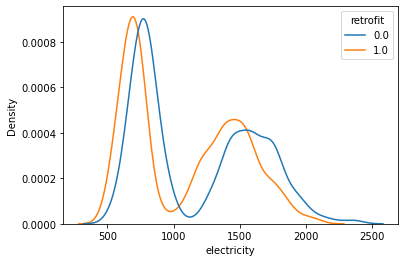
\includegraphics[scale = 0.7]{kdeplot.png}
    \caption{Treated households shown in orange}

\end{figure}

\end{document}